\subsubsection{その他の方法}

その他にも、多くの設計方法がある。反復型・適応型の方法では、厳密な要求と設計を最初にすべて固定するのではなく、ソフトウェア増分を作りながら設計を調整する。

\term{サービス指向設計}{Service-Oriented Design} は、分散されたサービスを組み合わせてソフトウェアを作る方法である。HTTP、HTTPS、SOAPなどの標準プロトコルを使い、異なる提供者のサービスをつなぐことがある。

\begin{figure}[htbp]
\centering
\IfFileExists{assets/fig-ch03-10.png}{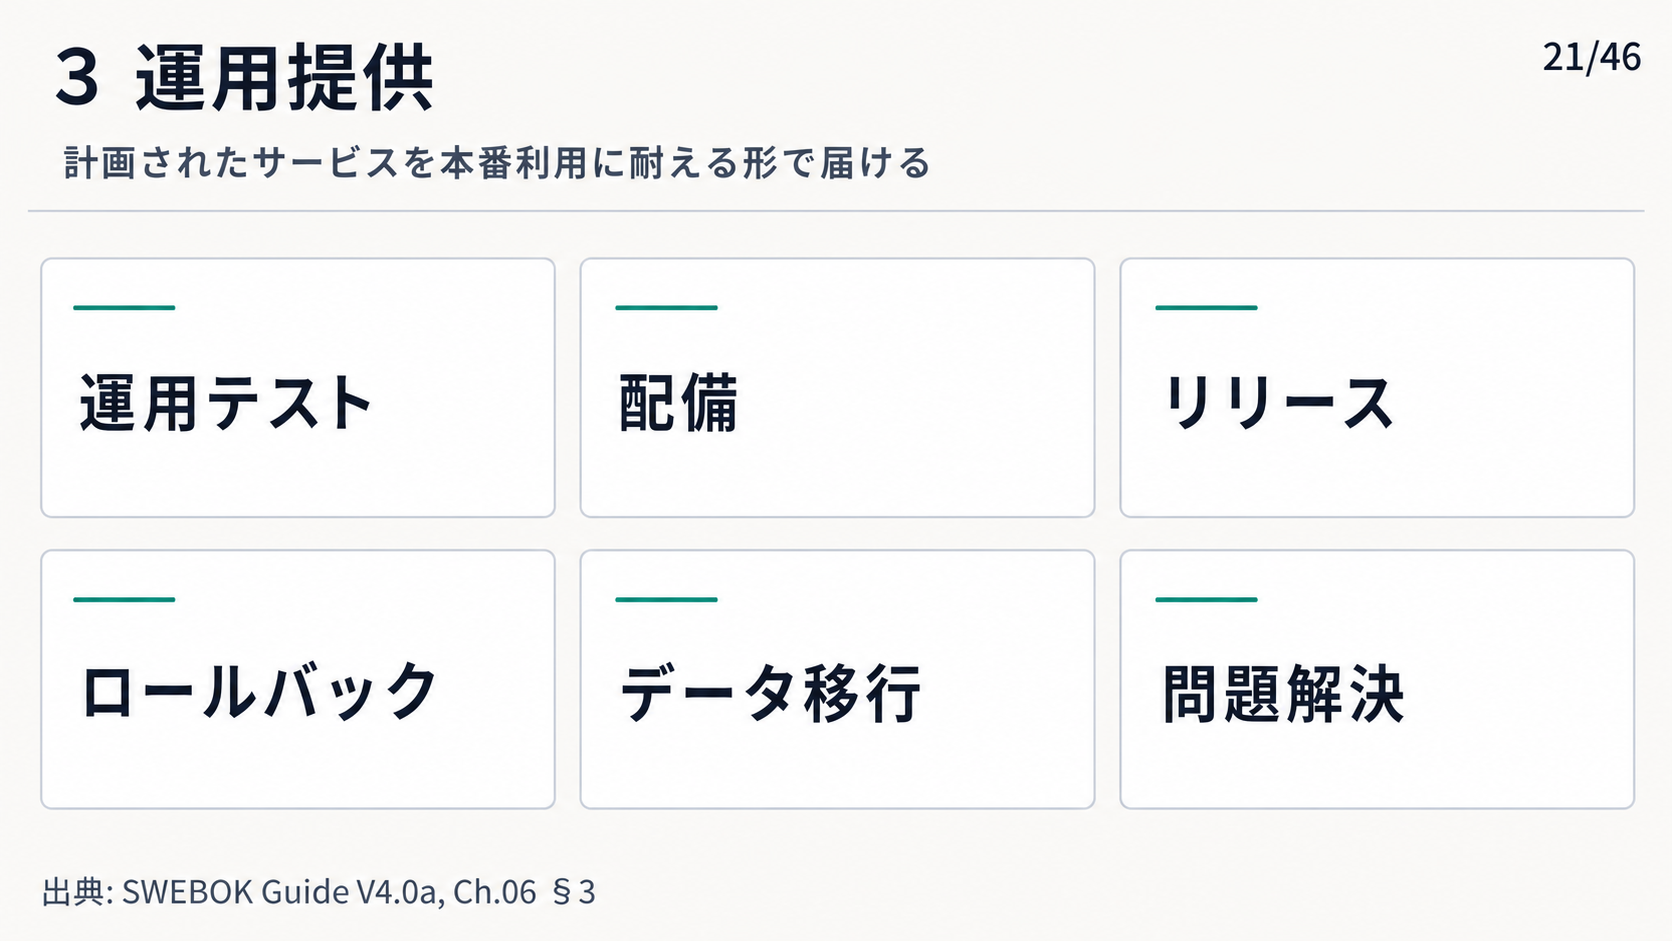
\includegraphics[width=0.96\linewidth]{assets/fig-ch03-10.png}}{\fbox{\parbox[c][48mm][c]{0.9\linewidth}{\centering 画像生成待ち\\設計戦略と中心概念の対応図}}}
\caption{設計戦略と中心概念の対応図}
\label{fig:ch03-10}
\end{figure}
